\documentclass[border=4pt]{standalone}
% Preámbulo común de las figuras. Cada figura es un documento standalone
% que se compila a SVG con scripts/build_figures.sh
\usepackage[utf8]{inputenc}
\usepackage{amsmath}
\usepackage{tikz}
\usepackage[american, siunitx]{circuitikz}
\usetikzlibrary{arrows.meta,calc,decorations.pathmorphing,patterns}
\tikzset{
  >={Stealth[length=2.2mm]},
  eje/.style={->, thin},
  hilo/.style={thick},
}
% Paleta común: tonos medios legibles sobre fondo claro
\definecolor{azul}{RGB}{31,94,168}
\definecolor{rojo}{RGB}{192,57,43}
\definecolor{verde}{RGB}{39,128,73}
\definecolor{naranja}{RGB}{211,120,30}
\definecolor{morado}{RGB}{125,60,152}

\begin{document}
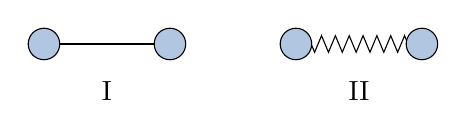
\begin{tikzpicture}[scale=1.0]
  \draw[thick] (0,0) -- (1.6,0);
  \fill[azul!35] (0,0) circle (0.2); \draw (0,0) circle (0.2);
  \fill[azul!35] (1.6,0) circle (0.2); \draw (1.6,0) circle (0.2);
  \node at (0.8,-0.6) {I};
  \draw[decorate, decoration={zigzag, segment length=5pt, amplitude=3pt, pre length=3pt, post length=3pt}] (3.2,0) -- (4.8,0);
  \fill[azul!35] (3.2,0) circle (0.2); \draw (3.2,0) circle (0.2);
  \fill[azul!35] (4.8,0) circle (0.2); \draw (4.8,0) circle (0.2);
  \node at (4.0,-0.6) {II};
\end{tikzpicture}
\end{document}
